\section{Knowledge Representation in the Semantic Web}
\label{sec:chp2_semweb}

This section describes the concepts that play a relevant role in knowledge representation on the Web, hence also relevant to its creation. First we present the Resource Description Framework (RDF)~\parencite{rdf}, used as backbone of knowledge graphs and also for specifying declarative transformation rules (\cref{sec:chp2_rdf}). Then, we discuss different approaches for annotating statements in RDF to add additional information (\cref{sec:chp2_reifications}).

\subsection{Resource Description Framework (RDF)}
\label{sec:chp2_rdf}

The Resource Description Framework (RDF)~\parencite{rdf} is a standard model for data interchange on the Web. Its basic unit are triples: two concepts linked by a relationship. These triples are represented in the form of $<$ \textit{s,p,o} $>$, where \textit{s} is the subject, \textit{p} is the predicate and \textit{o} the object. This model relies on the use of the linking structure of the Web, using IRIs to identify uniquely every resource and relationship. 

\cref{lst:chp2_rdf-example} presents an example of an RDF graph composed of a set of triples about pole vault records, which is also visually depicted in \cref{fig:chp2_rdf-example}. In total there are four triples. They all share the same subject, which is a resource uniquely identified by the IRI $<$\texttt{http://example.com/athlete/1}$>$. Likewise, all predicates in the triples are also defined by an IRI, e.g. $<$\texttt{http://example.com/ns\#name}$>$. The first triple (Line 5) defines that the subject is an instance of the class \texttt{ex:Athlete} with the predicate \texttt{rdf:type}. The rest of the triples define attributes of this instance with name (\texttt{ex:name}) and position in the ranking (\texttt{ex:rank}). The objects of both triples are literals, that may be strings ("Yelena Isinbayeva", Line 6) or typed literals ("1"\scalebox{.8}{\textsuperscript{$\wedge\wedge$}}\texttt{xsd:integer}, Line 7). Type literals refer to data values attached with a tag that represents their data type.

\begin{minipage}{\textwidth}
\begin{captionedlisting}{lst:chp2_rdf-example}{Example of RDF graph in Turtle serialization.}
\centering
{\begin{lstlisting}[language=r2rml]
@prefix rdf: <http://www.w3.org/1999/02/22-rdf-syntax-ns#>.
@prefix xsd: <http://www.w3.org/2001/XMLSchema#>.
@prefix ex: <http://example.com/ns#>.

<http://example.com/athlete/1> rdf:type ex:Athlete .
<http://example.com/athlete/1> ex:name "Yelena Isinbayeva" .
<http://example.com/athlete/1> ex:rank "1"^^xsd:integer .
\end{lstlisting}}
\end{captionedlisting}
\end{minipage}

There are different syntaxes to serialize RDF graphs. RDF/XML\footnote{\url{https://www.w3.org/TR/rdf-syntax-grammar}} was the first to be proposed, and relies on XML. Notation3 (N3)\footnote{\url{https://www.w3.org/TeamSubmission/n3/}} was developed as a human readable syntax, but its use is not common. Instead, the N-Triples\footnote{\url{https://www.w3.org/TR/n-triples}} and Turtle\footnote{\url{https://www.w3.org/TR/turtle}} serializations, subsets of N3, are more widely used. JSON-LD\footnote{\url{https://www.w3.org/TR/json-ld11}} was developed for programming environments, as it is written in JSON documents. Lastly, RDFa\footnote{\url{https://www.w3.org/TR/rdfa-primer}} extends HTML to markup structured content in webpages, with the objective of improving the results retrieved by search engines. 



\begin{figure*}[t]
\centering
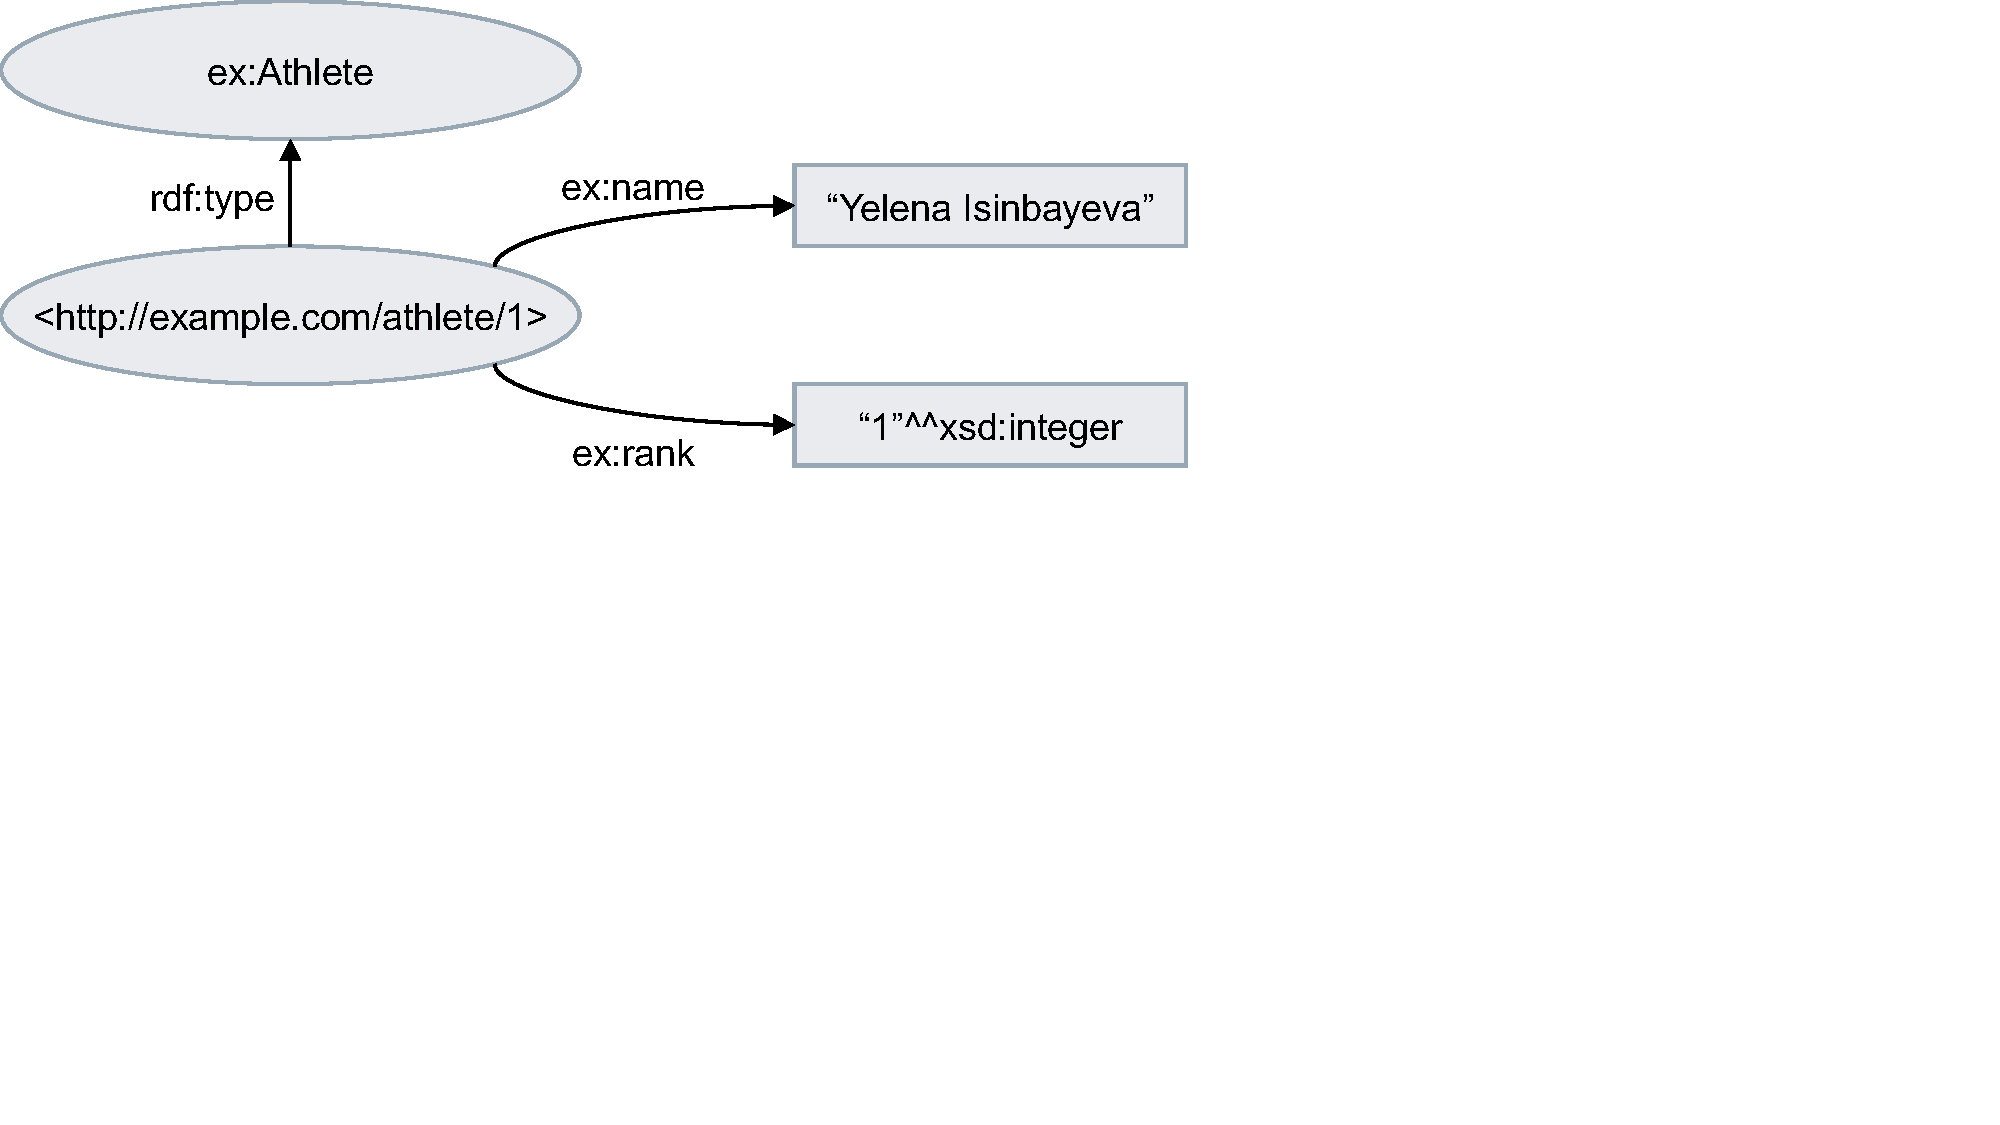
\includegraphics[width=0.6\linewidth]{figures/chp2_rdf-example.pdf}
\caption[RDF graph example]{Visual representation of the RDF graph shown in \cref{lst:chp2_rdf-example}.}
\label{fig:chp2_rdf-example}
\end{figure*}

\subsection{Statements about statements in RDF}
\label{sec:chp2_reifications}

%\ana{basic intro about what is this for and mot example about info that cannot be plainly represented in RDF. Then present all approaches used along the document: std reification, n-ary relationships, singleton properties, rdf-star, named graphs, i'd leave wikidata out of this}

Plain triples are not always able to represent the complexity of all knowledge. This is the case of statement annotation, when it is required to add information to a triple that does not correspond to a single resource, but the entire statement. This situation triggered the development of different approaches to enable triple annotation (also known as reification). \cref{fig:chp2_reification} illustrates instances of these models for the main statement \textit{Yelena Isinbayeva obtained the first position in the rank}, annotated with the additional statement \textit{in the season of 2009}. 

\begin{figure*}[t]
\centering
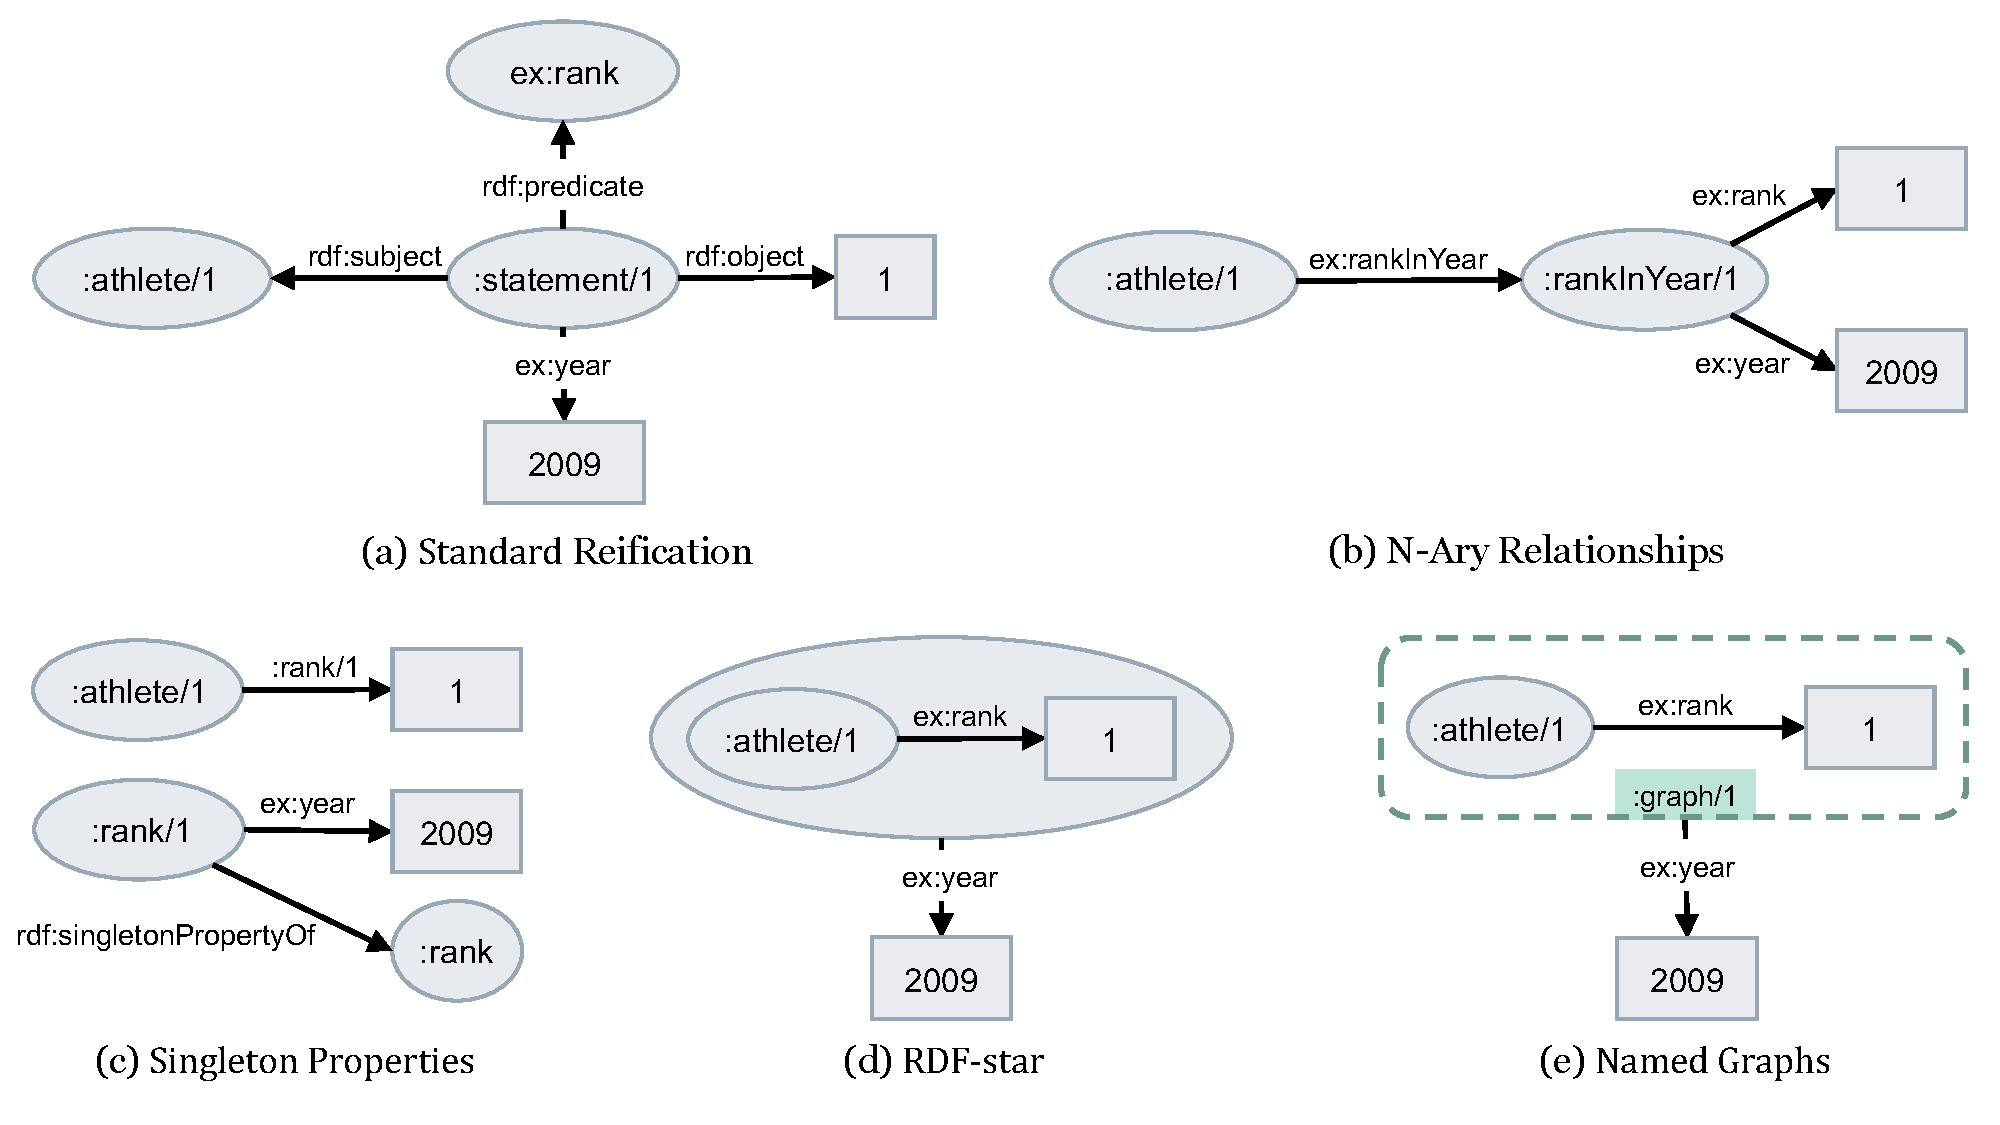
\includegraphics[width=\linewidth]{figures/chp2_reifications.pdf}
\caption[Approaches for statement reification in RDF]{Approaches for statement reification in RDF: (a) Standard Reification, (b) N-Ary Relationships, (c) Singleton Properties, (d) RDF-star and (e) Named Graphs.}
\label{fig:chp2_reification}
\end{figure*}

\noindent\textbf{Standard Reification}~\parencite{lassila1999rdf} explicitly declares a resource to denote an \texttt{rdf:Statement}.
This statement has \texttt{rdf:subject}, \texttt{rdf:predicate}, and \texttt{rdf:object} attached to it and can be further annotated with additional statements. The resource is typically a blank node, but an IRI can be used. 
In \cref{fig:chp2_reification}a, the resource \texttt{:statement/1} is an \texttt{rdf:Statement} with four associated triples, where the objects of the triples are the actual values of the triple (i.e. \texttt{:athlete/1} for the subject, \texttt{ex:rank} for the predicate, and \texttt{1} for the object). The property \texttt{ex:year} is used with its own value as object.


\noindent\textbf{N-Ary Relationships}~\parencite{naryw3c2006} converts a relationship into an instance that describes the relation, which can have attached both the main object and additional statements.
This representation is widely used in ontology engineering as an ontology design pattern~\parencite{gangemi2013multi}. In \cref{fig:chp2_reification}b, the entity \texttt{:athlete/1} points to an intermediate node (\texttt{:rankInYear/1}) which holds the triples for both the position in rank and year when it took place.

\noindent\textbf{Singleton Properties}~\parencite{nguyen2014don} uses unique predicates in the main triple. This unique predicate can then become the subject of the additional triple. The unique predicate is linked to the original predicate using \texttt{rdf:singletonPropertyOf}.
In \cref{fig:chp2_reification}c, the main triple uses the predicate \texttt{:rank/1}, the unique version of the original \texttt{ex:rank}. This predicate is then annotated with the year of the ranking. 

\noindent\textbf{RDF-star}~\parencite{hartig2017foundations,hartig2023rdf} extends RDF with a new syntax for compact triple reification. 
It introduces the notion of triple recursiveness with \texttt{Quoted Triples}, which can be used as subjects and/or objects of other triples. This is the only approach that extends the standard RDF features. 
%, having a potential impact on the development of supporting tools, triplestores, etc. 
This representation is currently being incorporated into the RDF 1.2 specification~\parencite{hartig2023rdf}, which is currently being developed under the RDF-star W3C Working Group\footnote{\url{https://www.w3.org/groups/wg/rdf-star/}}.
In Figure \ref{fig:chp2_reification}d we observe the example as an RDF-star graph, and it is represented in RDF as \texttt{{<<:athlete/1 ex:rank 1>> ex:year 2009}}.


\noindent\textbf{Named Graphs}~\parencite{rdf} are a SPARQL 1.1 feature that allows the assignment of an IRI to one or several triples as a graph identifier. Hence, graph IRIs allow the unique identification of triples. These IRIs can be used as subjects to add additional statements. 
In \cref{fig:chp2_reification}e, the main triple indicating the rank position of an athlete is assigned the named graph \texttt{:graph/1}. The graph IRI is subsequently used as subject in a triple that adds information about the year of the triple within the graph. 